\chapter{Разработка онтологических моделей,  методик наполнения и анализа образовательных данных в системе дистанционного обучения} \label{chapt3}




\section{Модель взаимодействия объектов системы дистанционного обучения} \label{sect3_1}

Данные в системе дистанционного обучения ECOLE хранятся в формате RDF(Resource Description Framework). Для хранения данных в системе был разработан набор онтологий. Модель данных системы делится на три основных уровня: уровень предметных областей, уровень учебных материалов, уровень деятельности пользователей в системе. Уровни модели связаны друг с другом для обеспечения взаимодействия различных ресурсов системы. Модель данных представлена на рисунке \ref{img:overall_model}.

\begin{figure} [h] 
  \center
  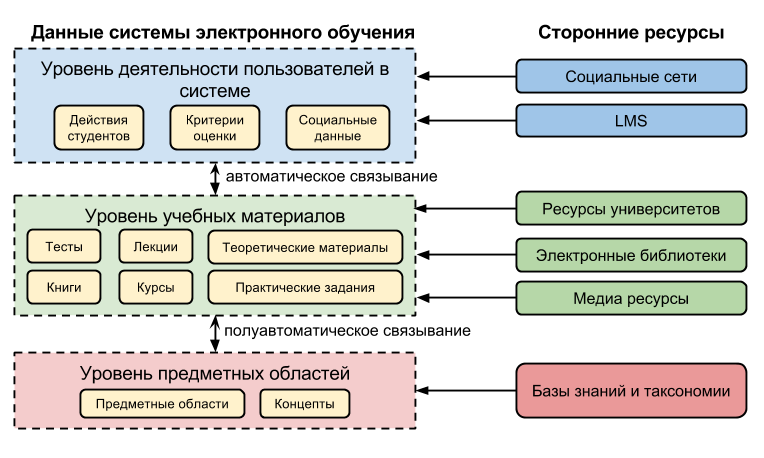
\includegraphics [scale=0.5] {overall_model}
  \caption{Общая модель данных системы дистанционного обучения ECOLE.} 
  \label{img:overall_model}  
\end{figure}

Уровень предметных областей является основой модели данных и содержит информацию о предметных областях науки и образования. Сбор данных для этого уровня производится из сторонних баз знаний, таксономий и опубликованных наборов данных таких как DBpedia и Mathematics Subject Classification. 

Уровень учебных материалов содержит информацию необходимую для проведения учебного процесса. Уровень содержит данные по образовательным программам, курсам, тестам и медиа ресурсам. Сбор данных для этого уровня производится из хранилищ университетов, открытых электронных библиотек и медиа ресурсов. Связывание учебных материалов с предметными терминами и областями производится в полуавтоматическом режим с использованием алгоритмов обработки естественного языка. 

Уровень деятельности пользователей в системе содержит результаты обучения студентов и  статистические данные по активности пользователей. Статистика ведется в системе управления обучением LMS(Learning Management System). При ведении статистики используется информация из социальных сетей. Связывание статистики и результатов обучения с учебными материалами происходит в автоматическом режиме алгоритмами LMS.




\section{Онтология учебных материалов} \label{sect3_2}

Онтология учебных материалов описывает отношения между курсами, модулями, лекциями, тестами, практиками и предметными терминами. Онтология основана на  «врехнеуровневых» онтологиях рекомендованных к использованию при описании учебных материалов.

The Academic Institution Internal Structure Ontology (AIISO) является онтологией описывающей внутреннюю организационную структуру образовательного процесса. AIISO предоставляет классы и свойства для описания курсов и модулей.

The Bibliographic Ontology(BIBO) является онтологией описывающей библиографические ресурсы. В онтологии учебных материалов BIBO используется для описания рекомендованной литературы, научных публикаций, методичек и монографий. 

The Ontology for Media Resources(MA-ONT) является онтологией описывающей медиа ресурсы. С помощью классов и свойств MA-ONT в онтологии учебных материалов производится связывание лекций с видео материалами.

Основными классами онтологии учебных материалов являются: Курс, Модуль, Лекция, Тест, Экзамен, Практика, Предметная область, Предметный термин и Ресурс. Онтология состоит из 32 классов, 42 объектных свойств и 13 свойств-значений. Модель онтологии учебных материалов представлена на рисунке \ref{img:ontology_edu}.

\begin{figure} [h] 
  \center
  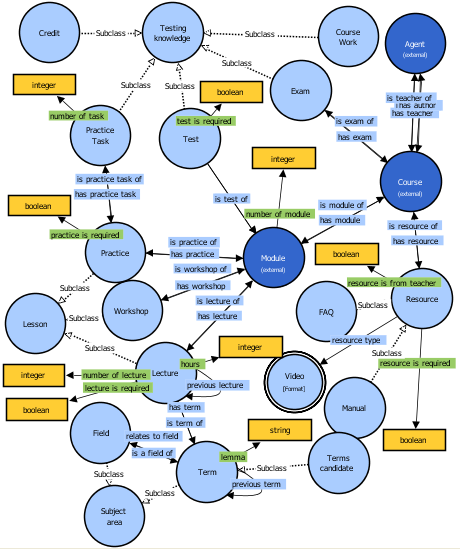
\includegraphics [scale=0.95] {ontology_edu}
  \caption{Основные классы и свойства онтологии учебных материалов.} 
  \label{img:ontology_edu}  
\end{figure}

В основе онтологии учебных материалов лежит модуль предметных терминов и областей. В данном модуле описываются отношения между терминами и объектами онтологии учебных материалов. В модуле описывается ряд вспомогательных классов и свойств для реализации методов гармонизации и анализа данных системы электронного обучения. Модель онтологии предметных терминов и областей представлена на рисунке \ref{img:ontology_term}.  

\begin{figure} [h] 
  \center
  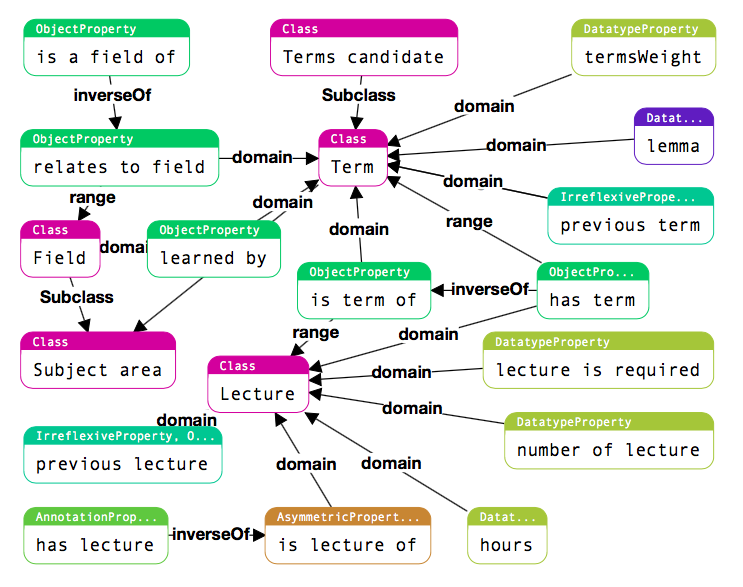
\includegraphics [scale=0.5] {ontology_term}
  \caption{Модель онтологии предметных терминов и областей.} 
  \label{img:ontology_term}  
\end{figure}

Одной из главных особенностей разработанной онтологии является возможность произведения прямого и косвенного междисциплинарного связывания объектов в курсах. Например тест по курсу физики «Интерференция и когерентность» включает в себя использование математических терминов таких как «Вектор» и «Векторное произведение». Если студент не сможет успешно пройти данный тест, система должна рекомендовать к повторению не только лекции по физики, но и определенные лекции по векторной алгебре. Данный пример демонстрирует косвенное связывание курсов физики и векторной алгебры с помощью предметных терминов «Вектор» и «Векторное произведение». Пример представлен на рисунке \ref{img:ontology_edu_example}. Связывание объектов курса с предметными терминами позволяет косвенно связывать лекции, тесты и методические материалы друг с другом.

\begin{figure} [h] 
  \center
  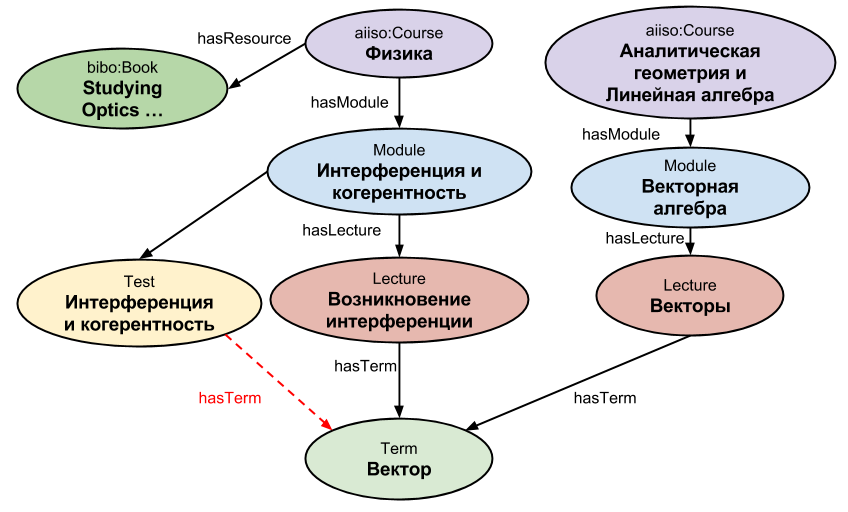
\includegraphics [scale=0.5] {ontology_edu_example}
  \caption{Пример косвенного связывания курсов с помощью предметных терминов.} 
  \label{img:ontology_edu_example}  
\end{figure}




\section{Онтология тестов} \label{sect3_3}

Для описания содержания тестов был разработана онтология тестов. Разработка онтологии производилась методом раскрытия и конкретизации существующих онтологий верхнего уровня. Именно по этому при разработке онтологии использовался нисходящий подход. Онтология тестов содержит классы описывающие тесты, группы и варианты вопросов, задания, ответы, вопросы, различные типы вопросов и ответов. Онтология содержит 12 классов, 10 объектных свойств и 6 свойств-значений. Основной целью онтологии тестов является представление структуры тестов и предоставление возможности автоматического семантического связывания заданий тестов с предметными терминами. Онтология описывает тест как набор из вариантов групп заданий. В каждой группе содержится набор заданий. Задания теста состоят из вопроса и набора ответов. В зависимости от типа вопроса у задания может быть различный набор правильных и неправильных ответов. Связывание предметных терминов с заданиями позволяет описать содержание вопроса и ответов задания.




\section{Онтология активности студента в системе обучения} \label{sect3_4}

Онтология активности студента в системе обучения была разработана для хранения информации о прогрессе и результатах обучения студентов в системе. При разработке были использованы две онтологии верхнего уровня: онтология тестов и онтология Friend Of A Friend (FOAF). Онтология FOAF используется для описания людей и отношений между ними. В дистанционной системе обучения FOAF может быть использована для описания персоналий студентов, преподавателей и других пользователей системы.

Онтология активности студента в системе обучения состоит из 10 классов, 15 объектных свойств и 5 свойств-значений. Основной задачей онтологии является хранение действий студентов в системе. В онтологию может быть записана информация о просмотре студентом видео-лекции, о прохождении теста или завершении курса. Онтология хранит в себе персональные данные студентов. В онтологию включены классы описывающие результаты студентов при прохождении тестов и изучении теоретического материала. Для хранения ответов на тесты конкретного студента используется связывание с онтологией тестов. Связи между студентами, их ответами на задания тестов и предметными терминами позволяют создавать косвенные связи между студентом и объектами курса. На основе полученных косвенных связей возможно реализация персонализированной рекомендательной системы для коррекции процесса обучения студентов. После прохождения теста студент может получить не только оценку, но и список предметных терминов и материалов для повторения составленный на основе ответов на тест.





\section{Онтология оценки знаний студента} \label{sect3_5}

Для реализации методов автоматизированной оценки рейтингов и знаний студентов предметных терминов и областей необходимо разработать и интегрировать в онтологическую модель системы модуль оценки знаний студентов. Модуль оценки знаний студентов - это онтология, которая позволяет хранить вычисленные автоматически оценки знаний студентов по определенным концептам и предметным областям. Онтологическая модель модуля оценки знаний студентов представлена на рисунке \ref{img:ontology_know}.

Онтология модуля содержит класс <<Rate>> (Оценка) и 5 подклассов, которые описывают следующие разновидности оценки:

\begin{itemize}
\item <<Lecture Term Rate>> - оценка предметного термина в контексте лекций; 
\item <<Test Attempt Term Rate>> - оценка предметного термина в контексте прохождения одного теста;
\item <<Average Test Term Rate>> - средняя оценка предметного термина за все тесты;
\item <<Total Term Rate>> - общая оценка предметного термина; 
\item <<Domain Rate>> - оценка предметной области. 
\end{itemize}

Каждый из классов оценки обладает свойством для хранения цифрового значения оценки <<value>>. Также онтология содержит объектные свойства для связывания объектов оценок с объектами студентов из модуля деятельности и результатов студента в системе обучения. В онтологии содержатся объектные свойства для связывания объектов тестов из модуля тестов с объектами терминов из модуля учебных материалов. Разработанная онтология позволяет добавлять новые классы оценок для хранения новых метрик при изменении алгоритмов расчета оценок.

\begin{figure} [h] 
  \center
  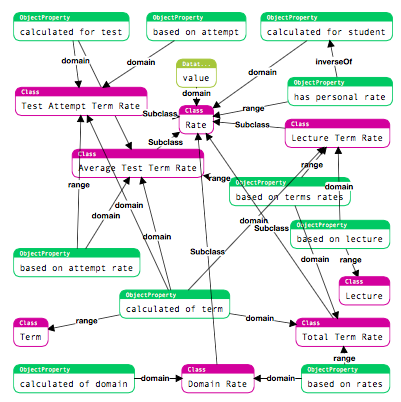
\includegraphics [scale=0.9] {ontology_know}
\caption{Онтологическая модель оценки знаний студентов.}
  \label{img:ontology_know}  
\end{figure}






\section{Метод интеграции учебных материалов из сторонних источников семантических данных} 
\label{sect3_6}

Технологии Semantic Web и Linked Data позволяют использовать онтологии для хранения, сбора и распространения данных. Одним из преимуществ данных технологий является повторное использование данных. В Интернете существует множество открытых источников с данными, при описании которых были использованы онтологии верхнего уровня. Данные источники могут быть использованы для наполнения системы дистанционного обучения. Автоматизация и разработка методов наполнения онтологий является одной из главных задач в реализации механизмов поддержки учебных материалов в актуальном состоянии в системе дистанционного обучения.

Для сбора данных в формате RDF в системе ECOLE используются провайдеры данных. Провайдеры данных поддерживают автоматическое обновление связных данных из сторонних источников. Провайдеры позволяют преобразовывать структурированные данных различных форматов в формат RDF. Каждый провайдер обладает своим контекстом для дальнейшего управления собранными данными. 

С помощью провайдеров данных система ECOLE наполняет онтологии учебных материалов и тестов. Система производит сбор данных из электронных библиотек. Одной из таких библиотек является The British National Bibliography(BNB). BNB предоставляет открытый доступ к библиографической информации в формате RDF. Библиографические данные описываются с помощью онтологии верхнего уровня BIBO. Система ECOLE собирает информацию о книгах и публикациях из BNB и предоставляет возможность преподавателям связывать их курсы с объектами BNB используя свойство «hasResource».

Система ECOLE позволяет задавать определения для предметных терминов. Одним из способов автоматизации наполнения онтологии терминов является использование внешней базы знаний. В системе ECOLE в качестве такой базы знаний используется DBpedia. DBpedia предоставляет точку доступа SPARQL для получения информации, которая была извлечена из Wikipedia. Провайдер данных автоматически создает определения для предметных терминов используя запросы к точке доступа SPARQL.

Множество источников в Интернете хранят структурированные данные не в формате RDF. Тесты и учебные материалы университета могут хранится в формате XML, а электронная библиотека предоставлять информацию о публикациях через REST API. Система ECOLE использует алгоритмы конвертации данных в провайдерах для интеграции структурированных данных в онтологии системы.




\section{Метод преобразования структурированных учебных материалов в семантический формат} \label{sect3_7}

%%%%%%%%%%%%%%%%%%%%%%%%%%%%%%%%%%%%%%%%%%%%%%%%%%

%%%%%         TODO

%%%%%%%%%%%%%%%%%%%%%%%%%%%%%%%%%%%%%%%%%%%%%%%%%%

\section{Использование алгоритмов обработки естественного языка для создания связей в онтологиях} \label{sect3_8}

Для наполнения онтологий системы можно использовать не только данные внешних источников, но и данные самой системы. Данные хранящиеся в онтологии системы и связанные семантическими связями позволяют создавать новые связи на основе предопределенных правил. Одним из методов связывания данных онтологии является применение алгоритмов обработки естественного языка NLP (Natural Language Processing). Используя данный подход можно извлекать семантические связи из текстовой информации объекта онтологии. Система ECOLE использует NLP алгоритмы для поиска предметных терминов в текстах заданий тестов.

Учитывая небольшой размер образца и предустановленный набор терминов,  шаблоны POS-tag в совместном использовании с синтаксическими шаблонами являются наиболее предпочтительным методом извлечения предметных терминов из заданий тестов[11][12][13]. Около десяти типичных составных шаблонов предметных терминов было использовано для извлечения терминов-кандидатов.  После извлечения термины-кандидаты приводились к канонической форме с использованием предустановленных словарей.

Для извлечения терминов была использована лингвистическая платформа NooJ[14]. NooJ обладает мощным механизмом регулярных выражений поиска, позволяющим комбинировать различные POS-tag шаблоны в единую грамматику для запроса к тексту. Для обработки русскоязычного текста авторами статьи был разработан набор грамматик и словарей. Данные словари и грамматики полностью покрывают словарь заданий теста. Для генерации словарей и грамматик для англоязычных ресурсов были использованы стандартные средства NooJ. Несколько деривационных парадигм было описано с помощью преобразователей NooJ и связано с лексическими сущностями. Применение деривационных парадигм позволяет генерировать основные леммы для лексических сущностей. Алгоритм извлечения предметных терминов из текста с использованием платформы NooJ состоит из следующих шагов:

\begin{itemize}
\item тест задания подгружается в платформу NooJ, что приводит к его лингвистическому анализу, используя разработанные словари;
\item в результате анализа платформа NooJ формирует текст с аннотациями, содержащими морфологическую и семантическую информацию о каждом слове;
\item применяя запросы на основе POS-tag шаблонов, платформа NooJ формирует список терминов-кандидатов.
\end{itemize}

Для применения алгоритма в других предметных областях и на других языках необходимо сформировать соответствующие словари, грамматики и шаблоны извлечения предметных терминов.

Для связывания терминов-кандидатов с предметными терминами системы с помощью лемм, термины системы должны пройти лемматизацию. Каждый предметный термин системы обладает свойством-значением <<lemma>>. Предметный термин системы хранит в данном свойстве все свои леммы.

Для реализации алгоритма связывания заданий тестов и предметных терминов был разработан провайдер данных. Провайдер принимает на вход ссылку на объект курса и производит создание ссылок между заданиями и терминами. Общий алгоритм работы провайдера данных представлен на рисунке \ref{img:nlp_main_alg}.

\begin{figure} [h] 
  \center
  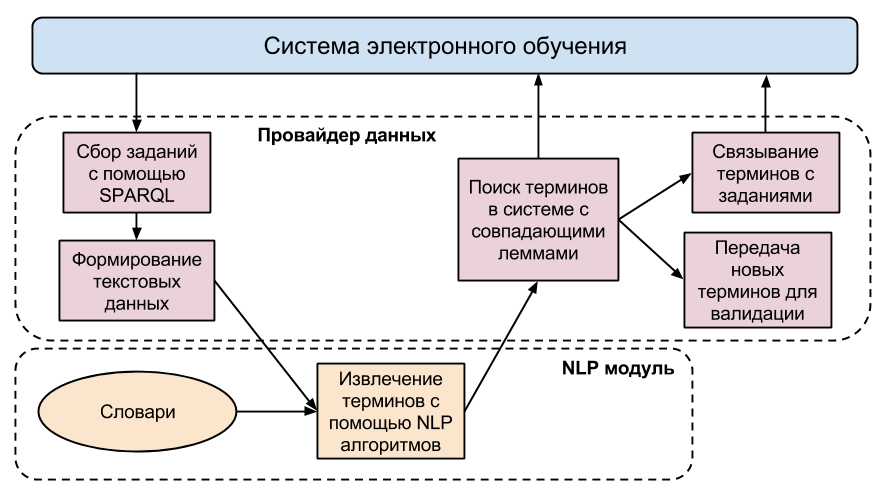
\includegraphics [scale=0.5] {nlp_main_alg}
\caption{Алгоритм работы провайдера извлечения терминов с использованием NLP алгоритмов.}
  \label{img:nlp_main_alg}  
\end{figure}

Алгоритм состоит из следующих шагов:

\begin{itemize}
\item провайдер собирает список заданий курса, используя запросы SPARQL;
\item происходит формирование текстовых данных для каждого задания, используя информацию о вопросах и ответах;
\item провайдер данных запускает NLP алгоритмы в платформе NooJ для текстовых данных каждого задания;
\item провайдер формирует список терминов-кандидатов содержащих каноническую форму и набор лемм;
\item производится поиск предметных терминов в системе с совпадающими наборами лемм для дальнейшего связывания с терминами кандидатами;
\item провайдер создает связи между найденными предметными терминами системы и заданиями терминов-кандидатов с помощью объектного свойства <<hasTerm>>.
\end{itemize}

Термины-кандидаты, для которых не были найдены соответствующие предметные термины системы, могут быть записаны в онтологию, как новые предметные термины системы. Перед записью в онтологию провайдер производит проверку термина-кандидата на соответствие предметному термину. Для проверки используются запросы к базе знаний DBpedia. В случае совпадения названия термина-кандидата со свойствами <<rdfs:label>> или <<dbpedia-owl:wikiPageRedirects>> объекта из Dbpedia, в онтологии системы создается новый предметный термин на основе термина-кандидата и производится связывание с заданиями теста. При отсутствии совпадений термин-кандидат помечается провайдером данных как ложный термин. При SPARQL запросах к базе знаний DBpedia используется фильтрация по предметным областям и категориям с помощью свойства <<dcterms:subject>>.

Данная фильтрация позволяет избежать ошибочных совпадений терминов-кандидатов с терминами из сторонних предметных областей. Проверка считается успешной в случае одного или более найденных совпадений для термина-кандидата. Для включения нового термина в систему необходима верификация преподавателя или администратора системы. Алгоритм проверки терминов-кандидатов представлен на рисунке \ref{img:nlp_check_alg}.

\begin{figure} [h] 
  \center
  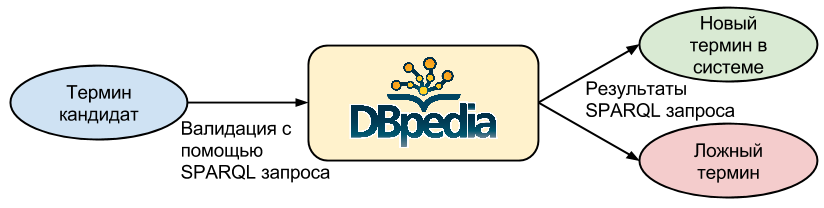
\includegraphics [scale=0.5] {nlp_check_alg}
\caption{Алгоритм проверки новых терминов-кандидатов.}
  \label{img:nlp_check_alg}  
\end{figure}


\section{Метод анализа качества учебных материалов основе свойств и связей в онтологиях и действий пользователей системы} \label{sect3_9}

Анализ качества учебных материалов производится внутри аналитических модулей системы. Каждый модуль состоит из отдельной аналитической страницы с графиками, таблицами и другими визуальными компонентами. Аналитические страницы основаны на синтаксисе Semantic MediaWiki и хранятся в платформе Information Workbench. Данные графиков, таблиц и визуальных элементов собираются аналитическим модулем с помощью SPARQL запросов к точке доступа.

Одним из примеров метода анализа качества учебных материалов является анализ покрытия лекций курса тестами и заданиями. В онтологии системы лекции и тесты связаны с определенным модулем курса. В результате работы алгоритмов по наполнению онтологий лекции и задания тестов могут быть связаны с определенными предметными терминами. Таким образов происходит косвенное связывание лекций и тестов через предметные термины. Система может предоставить статистику по количеству предметных терминов лекций модуля использованных в тестах модуля. Если термин лекции использован в задании теста, он считается покрытым в данном модуле. Каждый модуль имеет аналитическую страницу. 

Аналитическая страница модуля содержит следующую статистическую информацию:

\begin{itemize}
\item количество покрытых и непокрытых предметных терминов в модуле,
\item общий процент покрытия модуля тестами на основе отношения покрытых терминов к общему количеству терминов,
\item облако тегов предметных терминов модуля демонстрирующее качество и степень покрытия каждого термина,
\item список непокрытых терминов модуля, которые были использованы в лекциях, но не были использованы в заданиях тестов.   
\end{itemize}

Интерфейс аналитической страницы модуля позволяет получать информацию о покрытии тестами каждой лекции в отдельности. Интерфейс представлен на рисунке \ref{img:anl_screen_cover}.

\begin{figure} [h] 
  \center
  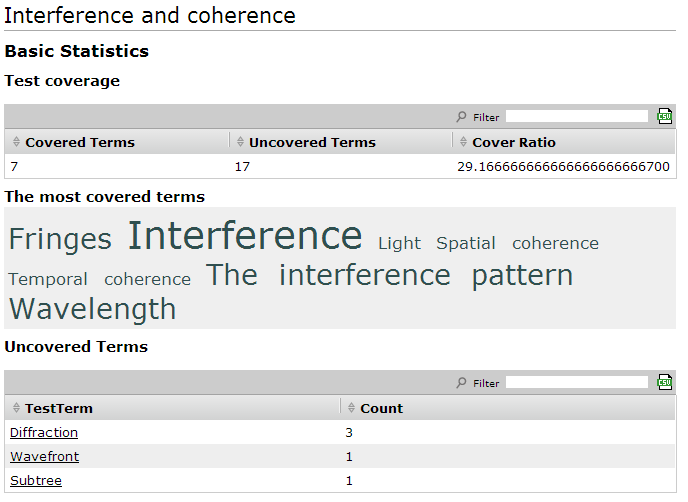
\includegraphics [scale=0.8] {anl_screen_cover}
\caption{Интерфейс статистики покрытия лекций тестами в аналитической странице модуля.}
  \label{img:anl_screen_cover}  
\end{figure}


Другим подходом к анализу учебных материалов является выявление проблемных предметных терминов в модуле курса. Проблемными предметными терминами являются термины, при изучении которых у студентов возникают наибольшие затруднения. Статистика по результатам прохождения студентами тестов, правильные и неправильные ответы на задания связанные с определенными предметными терминами позволяют рассчитать рейтинг знания каждым студентом определенного термина. Используя данный рейтинг, преподаватель, может получить список предметных терминов курса, которых студенты знают хуже всего. Это позволит преподавателю вносить коррективы в учебные материалы и учебный процесс. В текущей реализации данного аналитического модуля рейтинг проблематичного термина рассчитывается делением количества неправильных ответов на количество правильных ответов на задания связанные с данным термином. В будущем данная формула будет усложнена с учетом сложности заданий и глобального рейтинга терминов студентов. Рейтинг проблемных терминов для модуля составляется с помощью следующего  SPARQL-запроса:

\begin{verbatim}
    SELECT ?term 
        (count(?correct_answer) AS ?correct_answer_count)
        (count(?answer) AS ?answer_count)
        ((2*?correct_answer_count - ?answer_count) 
            AS ?rank) 
    WHERE{
        ?module learningRu:hasTest ?test  . 
        ?test ifmotest:hasGroupOfTasks 
            ?group_of_tasks .        
        ?group_of_tasks ifmotest:hasTask ?task .      
        ?test_element lres:hasTask ?task .
        ?test_element lres:hasAnswer ?answer .
        ?task learningRu:hasTerm ?term .       
        OPTIONAL { 
            ?task ifmotest:hasCorrectAnswer 
                ?correct_answer
            filter( ?correct_answer = ?answer)
        }         
    }
    GROUP BY ?term 
    ORDER BY ASC(?rank)
\end{verbatim}

Анализ проблемных терминов реализован на аналитической странице модуля. Аналитическая страница модуля включает в себя список проблемных терминов с рейтингами и диаграмму отношений между пятью самыми проблемными терминами модуля.

Аналитика учебного материала, основанная на использовании семантических связей между объектами системы, позволяет строить различные запросы для оценки качества учебных материалов. Полученная информация позволяет преподавателям и авторам курса выявлять и исправлять устаревшие, ошибочные и неточные учебные материалы, основываясь на динамике образовательного процесса и его структуре.



\section{Автоматизированная оценка знаний студентов на основе анализа онтологий} \label{sect3_10}

Подход к автоматизированному анализу знаний и рейтингов студентов системы электронного обучения основан на семантическом анализе действий студентов в системе электронного обучения в проекции образовательного процесса и учебных материалов. Целью подхода является автоматизированный вывод рейтинга знаний студента по определенной предметной области учебной дисциплины. Рейтинг знания предметной области зависит от рейтингов входящих в нее предметных терминов. Расчет рейтинга знания предметного термина зависит от метрик оценки действий студента в системе. Набор метрик может варьироваться в зависимости от возможных действий студентов в системе, структуры онтологии и необходимой точности вычислений. В предложенном подходе используются метрики: метрика знакомства с термином и метрика проверки знания термина с помощью тестов. Расчет рейтинга знаний предметной области производится с учетом значения(важности) предметных терминов в образовательном процессе.

Рейтинг знания термина, как и рейтинг знания предметной области, варьируется от 0 до 1. Метрика знакомства с термином является бинарной метрикой и обозначает факт изучения студентом предметного термина с использованием теоретического материала. В разработанном подходе изучением предметного термина является завершение студентом лекции связанной с данным термином в системе электронного обучения. Изучить предметный термин студент может только один раз. В разработанном подходе данная метрика составляет 15\% от общего рейтинга знаний предметного термина.

Метрика проверки знания предметного термина с помощью тестов основана на статистическом анализе правильных и неправильных ответов студента на задания учебных курсов, которые связаны с данным термином. В разработанном подходе данная метрика составляет 85\% от общего рейтинга знаний предметного термина. Метрика рассчитывается как нижняя граница доверительного интервала Вильсона для параметра Бернулли по количеству правильных и неправильных ответов, используя формулу:

$$
    R_t = \frac{p+\frac{1}{2n}z_{1-\alpha/2}^2 \pm z_{1-\alpha/2}\sqrt{\frac{p(1-p)}{n}+\frac{z_{1-\alpha/2}^2}{4n^2}}{} }{1+\frac{1}{n}z_{1-\alpha/2}^2},
$$

где \(z_{1-\alpha/2}\) - квантиль от от \(1-\alpha/2\) стандартного нормального распределения, \(p\) - доля правильных ответов, \(n\) - общее количество ответов. 

Сумма двух полученных метрик для предметного термина в соответствии с их долями является общим рейтингом знания предметного термина. Предметные области и предметные термины в соответствии с разработанной моделью не зависят от учебных материалов и могут повторно использоваться во множестве учебных курсов. Связи между терминами, описывающие необходимость одного термина для изучения другого, позволяют рассчитать значение предметного термина в образовательном процессе. Чем больше предметных терминов, для изучения которых необходим определенный термин, тем выше значение данного термина. При расчете учитывается количество терминов на разных уровнях зависимости. Уровнем зависимости является глубина косвенной зависимости одного термина от другого через набор терминов. Например, на втором уровне зависимости находятся термины, зависимые от предметных терминов, зависимых от рассматриваемого предметного термина. Значение термина рассчитывается с использованием трех уровней зависимости по формуле: 

$$
    W_t = \frac{1}{e}+\sum_{k=1}^{3}\frac{n_k}{e^k}, 
$$

где \(n\) - количество терминов, связанных с данным термином на каждом уровне зависимости, \(k\) - номер зависимого уровня, \( \frac{1}{e} \) - константное значение термина. 

Итоговый рейтинг знания студентом предметной области учебной дисциплины рассчитывается как сумма рейтингов предметных терминов, входящих в предметную область. При расчете необходимо учитывать относительное значение термина в предметной области. Для этого необходимо рассчитать суммарное значение предметной области, используя формулу:

$$  
    W_f = \sum_{n=1}^{\infty}W_t,
$$

где \(W_t\) - значение предметного термина, \(n\) - количество терминов в предметной области.

Относительное значение термина в предметной области рассчитывается по формуле:

$$
    D_t = \frac{W_t}{W_f},
$$

где \(W_t\) - значение термина, \(W_f\) - значение предметной области.

Рейтинг предметной области является суммой рейтингов предметных терминов в соответствии с их относительными значениями:

$$
    R_f = \sum_{n=1}^{\infty} R_tD_t,
$$
где \(R_t\) - рейтинг термина, \(D_t\) - относительное значение термина в предметной области.

Представленный подход позволяет производить автоматизированную оценку знания студентами предметных областей. Поддержка набора метрик позволяет системе варьировать алгоритмы расчета оценки, добавляя, изменяя и удаляя необходимые метрики. Помимо оценки предметных областей данный подход можно применять к любым объектам образовательного процесса, напрямую или косвенно связанным с предметными терминами. Подход позволяет производить оценку учебных курсов и специальностей.

\clearpage
